\chapter{Graphically Solving Linear Programs}\footnote{Portions of this chapter are adapted from Kevin Cheung's \emph{A First Course in Linear Programming} materials (Carleton University), licensed CC BY-SA 4.0, with modifications by Robert Hildebrand. See the Sources and Attribution chapter for details.}

\begin{outcome}
\begin{enumerate}
\item[A.] Draw the region of points allowed by the constraints, together with level lines of the objective.
\item[B.] Locate the corner points of that region and compute their coordinates.
\item[C.] Read an optimal solution directly off the picture.
\item[D.] Recognize the four ways a linear program can turn out: a single best point, a whole edge of best points, no allowed points at all, or an objective that grows without limit.
\end{enumerate}
\end{outcome}
\begin{resource}
\begin{itemize}
\item \href{https://www.youtube.com/watch?v=K7TL5NMlKIk&ab_channel=Dr.TreforBazett}{Youtube! - Modeling with Linear Programming - Watch 4:20 - End}
\item \href{https://www.youtube.com/watch?v=E72DWgKP_1Y&t=1014s&ab_channel=TomS}{Youtube! - Watch 1:43 - 3:43}
\end{itemize}
\end{resource}

\begin{tryit}
\vizlink{objective-slider}{Objective-Level Slider}: drag the objective line across the feasible region and watch where optima land.
\end{tryit}


A linear program with two decision variables fits entirely on a sheet of paper: each constraint cuts the plane with a line, the points surviving every cut form the feasible region, and the objective becomes a family of parallel lines, one for each possible objective value. Sliding a line from this family across the region and watching where it exits gives a purely visual way to locate a best possible point, and this picture is the subject of the present chapter.

Our starting point is a small, well-behaved example whose picture is easy to draw.  Once its geometry is understood, we move on to examples where things go wrong in instructive ways.

%% Decorative LP images removed (files not available)

\section{Nonempty and Bounded Problem}\label{sec:nonempty-bounded}

Consider the problem
\begin{align*}
\max \quad & 2 x_1+5 x_2 \\
\text { s.t. } \quad
&x_1+2 x_2 \leq 16 \\
&5 x_1+3 x_2 \leq  45 \\
&x_1, x_2  \geq 0
\end{align*}

The first step is a picture of the \emph{feasible region}: every point $(x_1, x_2)$ that survives all of the constraints at once.

A reliable way to draw it is boundary-first: sketch the line where each constraint holds with equality, namely
\begin{itemize}
\item $x_1+2 x_2 = 16$
\item $5 x_1+3 x_2 = 45$
\item $x_1 = 0$
\item $x_2= 0$
\end{itemize}
and then shading in the side of the space cut out by the corresponding inequality.

\begin{figure}[h!]
\begin{center}
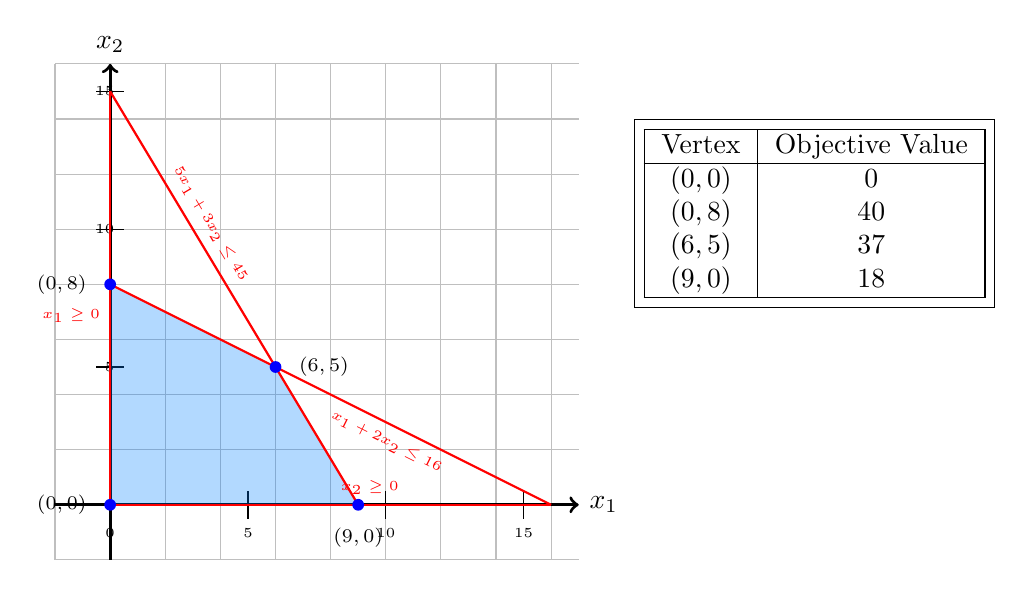
\begin{tikzpicture}[scale = 0.35]
    % Grid and axes
    \draw[gray!50, thin, step=2] (-2,-2) grid (17,16);
    \draw[very thick,->] (-2,0) -- (17,0) node[right] {$x_1$};
    \draw[very thick,->] (0,-2) -- (0,16) node[above] {$x_2$};

    % Axis labels
    \foreach \x in {0,5,10,15} \draw (\x,0.5) -- (\x,-0.5) node[below] {\tiny\x};
    \foreach \y in {0,5,10,15} \draw (-0.5,\y) -- (0.5,\y) node[left] {\tiny\y};

    % Shaded feasible region
    \fill[blue!50!cyan,opacity=0.3] (0,0) -- (0,8) -- (6,5) -- (9,0) -- cycle;

    % Constraint lines
    \draw[red,thick] (0,8) -- node[below right,sloped] {\tiny$x_1 + 2x_2 \leq 16$} (16,0);
    \draw[red,thick] (0,15) -- node[above left,sloped] {\tiny$5x_1 + 3x_2 \leq 45$} (9,0);
    \draw[red,thick] (0,0) -- node[below left] {\tiny$x_1 \geq 0$} (0,15);
    \draw[red,thick] (0,0) -- node[above right] {\tiny$x_2 \geq 0$} (16,0);

    % Vertices
    \node[blue] at (0,0) [circle,fill,inner sep=1.5pt]{};
    \node[blue] at (0,8) [circle,fill,inner sep=1.5pt]{};
    \node[blue] at (6,5) [circle,fill,inner sep=1.5pt]{};
    \node[blue] at (9,0) [circle,fill,inner sep=1.5pt]{};

    % Labels for vertices
    \node[black,anchor=east] at (-0.5,0) {\scriptsize$(0,0)$};
    \node[black,anchor=east] at (-0.5,8) {\scriptsize$(0,8)$};
    \node[black,anchor=west] at (6.5,5) {\scriptsize$(6,5)$};
    \node[black,anchor=north] at (9,-0.5) {\scriptsize$(9,0)$};
% Table within the TikZ picture
    \node[draw,fill=white,anchor=north west] at (19,14) {
        \begin{tabular}{|c|c|}
        \hline
        Vertex & Objective Value \\
        \hline
        $(0,0)$ & $0$ \\
        $(0,8)$ & $40$ \\
        $(6,5)$ & $37$ \\
        $(9,0)$ & $18$ \\
        \hline
        \end{tabular}
    };
\end{tikzpicture}
\end{center}
\caption{\href{https://www.desmos.com/calculator/j1li4l7lcv}{Desmos: Interactive plot!} (\href{https://open-optimization.github.io/open-optimization-or-book/interactive-figures/lp-graphical-method.html}{backup interactive plot})}
\end{figure}

Each line splits the plane in two; keeping the correct side of every line and shading whatever survives produces the feasible region.

Two features of this particular region are worth naming.  It is \emph{nonempty}: at least one point satisfies every constraint.  And it is \emph{bounded}: the whole region fits inside some large circle, with no direction in which it stretches forever.

The corners of the region, called \emph{extreme points}, will turn out to carry all the information we need about optimal solutions.  Each corner sits where two of the boundary lines cross, so corner coordinates come from solving $2 \times 2$ linear systems.  Watch out, though: crossing two boundary lines is necessary but not sufficient, since two lines can also intersect at a point that violates some third constraint.

We will later use the terminology \emph{basic feasible solution} for an extreme point of the feasible region, and \emph{basic solution} as a point that is the intersection of 2 lines, but is actually infeasible (does not satisfy all the constraints).

\begin{theorem}{Optimal Solution at a Vertex}\label{thm:optimalextremepoint}
If the feasible region of the linear program is nonempty and bounded, then there exists an optimal solution at a vertex of the feasible region.
\end{theorem}

This theorem implies the following algorithm.
\begin{algorithm}[H]
\caption{Enumerate Vertices Algorithm for Solving a Linear Programming Problem}
\label{alg:EnumerateVertices}
\begin{enumerate}
    \item \textbf{Identify the Feasible Region:}
    Determine the set of constraints defining the feasible region in the problem.
    \item \textbf{Enumerate Vertices:}
    Find all the vertices (corner points) of the feasible region. This can be done by solving pairs of constraint equations to find their intersections, keeping only those that satisfy all constraints.
    \item \textbf{Compute Objective Values:}
    Evaluate the objective function at each vertex of the feasible region.
    \item \textbf{Compare Objective Values:}
    For a maximization problem, identify the vertex with the highest objective value. For a minimization problem, identify the vertex with the lowest objective value.
    \item \textbf{Determine the Optimal Solution:}
    The vertex with the optimal objective value is the solution to the linear programming problem.
\end{enumerate}
\end{algorithm}

We will explore why Theorem~\ref{thm:optimalextremepoint} is true, and also what happens when the feasible region does not satisfy the assumptions of either nonempty or bounded.

\section{Graphical Approach}\label{sec:graphical-approach}
We now apply the vertex enumeration idea graphically using a concrete example.

\begin{example}{Furniture Workshop}\label{ex:FurnitureWorkshop}
A small furniture workshop produces chairs and tables. Each chair requires 2 hours of carpentry and 1 hour of finishing, earning a profit of \$8. Each table requires 1 hour of carpentry and 3 hours of finishing, earning a profit of \$6. The workshop has 80 hours of carpentry time and 90 hours of finishing time available per week. Market demand limits chair production to at most 32 per week.

Letting $x_1$ denote the number of chairs and $x_2$ the number of tables, the linear program is:
\begin{equation}
\begin{aligned}
\max\;\;& z(x_1,x_2) = 8x_1 + 6x_2\\
\text{s.t.}\;\;&  2x_1 + x_2 \leq 80\\
& x_1 + 3x_2 \leq 90\\
& x_1 \leq 32\\
& x_1 \geq 0\\
& x_2 \geq 0
\end{aligned}
\label{eqn:FurnitureWorkshop}
\end{equation}
\end{example}

\begin{solution} To solve graphically, we first sketch the feasible region by plotting the boundary lines of each constraint and shading the region that satisfies all inequalities simultaneously. The result is shown in Figure~\ref{fig:FurnitureWorkshopFeasibleRegion}.

\begin{figure}[H]
\centering
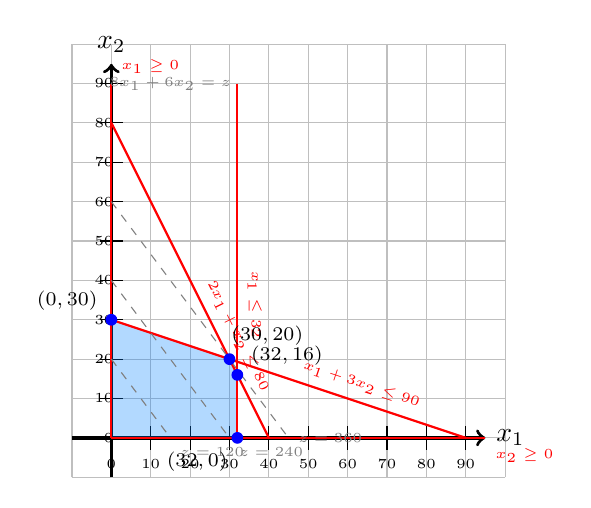
\begin{tikzpicture}[scale=0.05]
    % Grid and axes
    \draw[gray!50, thin, step=10] (-10,-10) grid (100,100);
    \draw[very thick,->] (-10,0) -- (95,0) node[right] {$x_1$};
    \draw[very thick,->] (0,-10) -- (0,95) node[above] {$x_2$};

    % Axis labels
    \foreach \x in {0,10,...,90} \draw (\x,3) -- (\x,-3) node[below] {\tiny\x};
    \foreach \y in {0,10,...,90} \draw (-3,\y) -- (3,\y) node[left] {\tiny\y};

    % Feasible region vertices: (0,0), (0,30), (30,20), (32,16), (32,0)
    \fill[blue!50!cyan,opacity=0.3]
        (0,0) -- (0,30) -- (30,20) -- (32,16) -- (32,0) -- cycle;

    % Constraint lines
    \draw[red,thick] (0,80) --  node[above right, sloped] {\tiny $2x_1 + x_2 \leq 80$}(40,0);
    \draw[red,thick] (0,30) --  node[above right, sloped] {\tiny $x_1 + 3x_2 \leq 90$}(90,0);
    \draw[red,thick] (32,90) --  node[above right, sloped] {\tiny $x_1 \leq 32$}(32,0);
    \draw[red,thick] (0,0) -- (95,0) node[below right] {\tiny $x_2 \geq 0$};
    \draw[red,thick] (0,0) -- (0,90) node[above right] {\tiny $x_1 \geq 0$};

    % Objective function contours (8x1 + 6x2 = z)
    \draw[dashed,gray] (0,120/6) -- (120/8,0) node[below right] {\tiny $z = 120$};
    \draw[dashed,gray] (0,240/6) -- (240/8,0) node[below right] {\tiny $z = 240$};
    \draw[dashed,gray] (0,360/6) -- (360/8,0) node[right] {\tiny $z = 360$};

    % Labels for vertices
    \node[blue] at (0,30) [circle,fill,inner sep=1.5pt]{};
    \node[blue] at (30,20) [circle,fill,inner sep=1.5pt]{};
    \node[blue] at (32,16) [circle,fill,inner sep=1.5pt]{};
    \node[blue] at (32,0) [circle,fill,inner sep=1.5pt]{};

    % Vertex coordinates
    \node[black,anchor=south east] at (-1,30) {\scriptsize $(0,30)$};
    \node[black,anchor=south west] at (28,21) {\scriptsize $(30,20)$};
    \node[black,anchor=south west] at (33,16) {\scriptsize $(32,16)$};
    \node[black,anchor=north east] at (32,-1) {\scriptsize $(32,0)$};

    % Objective function label
    \node[gray] at (15,90) {\tiny $8x_1 + 6x_2 = z$};
\end{tikzpicture}
\caption{Feasible region and level curves for the Furniture Workshop problem. The shaded polygon represents the set of all $(x_1,x_2)$ satisfying every constraint. Dashed lines show the objective function at several values of $z$. As $z$ increases, the level curves sweep upward and to the right.}
\label{fig:FurnitureWorkshopFeasibleRegion}
\end{figure}

Next, we overlay level curves of the objective function. Setting $8x_1 + 6x_2 = z$ gives the family of lines
\[
x_2 = -\tfrac{4}{3}\,x_1 + \tfrac{z}{6},
\]
which are parallel lines with slope $-4/3$. Increasing $z$ shifts them in the direction of the gradient $\nabla z = (8,6)$.  Sweeping the level curves in this direction, the last one to touch the feasible region does so at the vertex $(x_1^*,x_2^*) = (30,20)$, yielding the optimal profit
\[
z^* = 8(30) + 6(20) = 360.
\]

This optimal point sits at the intersection of the two constraints $2x_1+x_2=80$ and $x_1+3x_2=90$. Both constraints are satisfied with equality at the optimum; we say they are \textit{binding}. The remaining constraints ($x_1\leq 35$, $x_1\geq 0$, $x_2\geq 0$) are satisfied strictly and are \textit{non-binding}.

This illustrates a general principle: when an optimal solution to a linear program exists, it occurs at a vertex of the feasible region, the intersection of several binding constraints.
\end{solution}

We can now state a preliminary algorithm for solving a two-variable LP with a bounded feasible region graphically.
\begin{stepbox}{algpivot}{\ding{192}\ Graphical Method 1: Bounded Region, Unique Optimum}
\begin{enumerate}[nosep]
\item Sketch the feasible region by plotting each constraint boundary and shading the intersection of all half-planes.
\item Draw several level curves of the objective function $z = c_1 x_1 + c_2 x_2$ for increasing values of $z$.
\item Sweep the level curves in the gradient direction $\nabla z = (c_1, c_2)$ until the last level curve that still touches the feasible region is found.
\item The vertex of the feasible region lying on this last level curve is the optimal solution.
\end{enumerate}
\end{stepbox}

\begin{example}{Lemonade Vendor}\label{exa:lemonadevendor}
Say you are a vendor of lemonade and lemon juice. Each unit of lemonade
requires 1 lemon and 2 litres of water. Each unit of lemon juice
requires 3 lemons and 1 litre of water. Each unit of lemonade gives a
profit of three dollars. Each unit of lemon juice gives a profit of two
dollars. You have 6 lemons and 4 litres of water available. How many
units of lemonade and lemon juice should you make to maximize profit?

If we let \(x\) denote the number of units of lemonade to be made and
let \(y\) denote the number of units of lemon juice to be made, then the
profit is given by \(3x + 2y\) dollars. We call \(3x + 2y\) the
objective function. Note that there are a number of constraints that
\(x\) and \(y\) must satisfy. First of all, \(x\) and \(y\) should be
nonnegative. The number of lemons needed to make \(x\) units of lemonade
and \(y\) units of lemon juice is \(x+3y\) and cannot exceed 6. The
number of litres of water needed to make \(x\) units of lemonade and
\(y\) units of lemon juice is \(2x+y\) and cannot exceed 4. Hence, to
determine the maximum profit, we need to maximize \(3x + 2y\) subject to
\(x\) and \(y\) satisfying the constraints \(x + 3y \leq 6\),
\(2x + y \leq 4\), \(x \geq 0\), and \(y \geq 0.\)

A more compact way to write the problem is as follows:
\[\begin{array}{rrcrll}
\text{maximize } & 3x & + & 2y & \\
\text{subject to}
& x & + & 3y & \leq & 6 \\
& 2x & +&  y & \leq & 4 \\
& x &  & & \geq & 0 \\
& & & y & \geq & 0. \\
\end{array}\]

\end{example}
\begin{solution}
We can solve this maximization problem graphically as follows. We first
sketch the set of $(x,y)$  satisfying the
constraints, called the feasible region, on the \((x,y)\)-plane. We then
take the objective function \(3x+2y\) and turn it into an equation of a
line \(3x+2y = z\) where \(z\) is a parameter. Note that as the value of
\(z\) increases, the line defined by the equation \(3x+2y=z\) moves in
the direction of the normal vector
$(3,2)$. We call this direction the
direction of improvement. Determining the maximum value of the objective
function, called the optimal value, subject to the constraints amounts to
finding the maximum value of \(z\) so that the line defined by the
equation \(3x+2y=z\) still intersects the feasible region.

\begin{figure}[H]
\centering
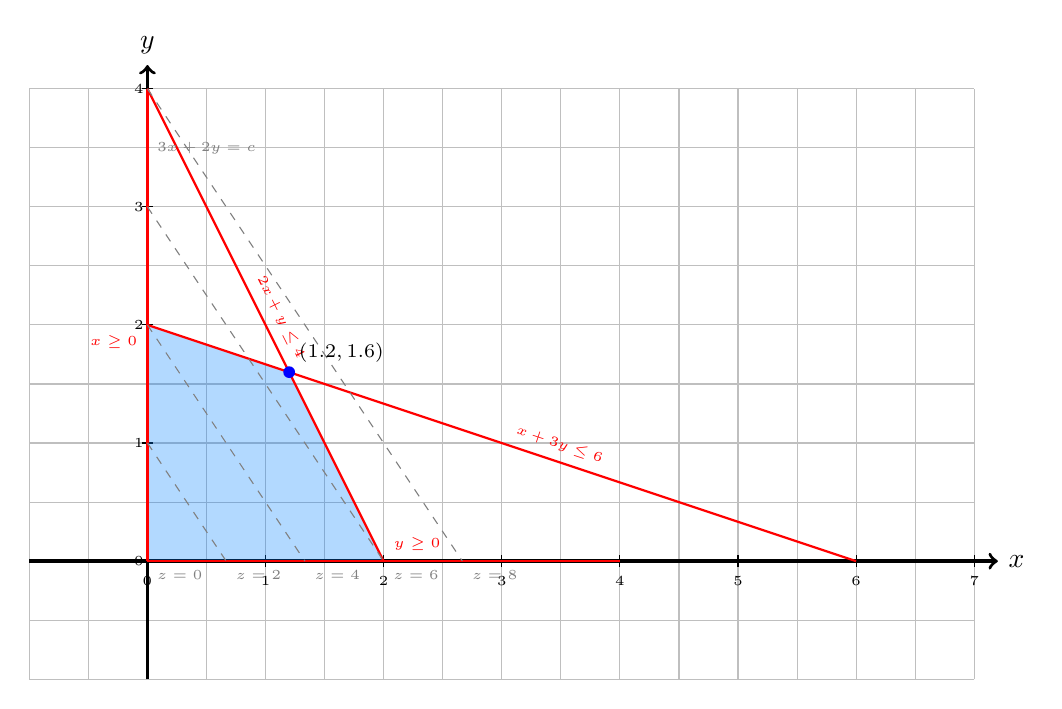
\begin{tikzpicture}[scale = 1.5]
    % Grid and axes
    \draw[gray!50, thin, step=0.5] (-1,-1) grid (7,4);
    \draw[very thick,->] (-1,0) -- (7.2,0) node[right] {$x$};
    \draw[very thick,->] (0,-1) -- (0,4.2) node[above] {$y$};

    % Axis labels
    \foreach \x in {0,...,7} \draw (\x,0.05) -- (\x,-0.05) node[below] {\tiny\x};
    \foreach \y in {0,...,4} \draw (-0.05,\y) -- (0.05,\y) node[left] {\tiny\y};

    % Shaded feasible region
    \fill[blue!50!cyan,opacity=0.3] (0,0) -- (0,2) -- (1.2,1.6) -- (2,0) -- cycle;

    % Constraint lines
    \draw[red,thick] (0,2) -- node[above right,sloped] {\tiny$x + 3y \leq 6$} (6,0);
    \draw[red,thick] (0,4) -- node[above,sloped] {\tiny$2x + y \leq 4$} (2,0);
    \draw[red,thick] (0,0) -- node[below left] {\tiny$x \geq 0$} (0,4);
    \draw[red,thick] (0,0) -- node[above right] {\tiny$y \geq 0$} (4,0);

        % Objective function contours
            \draw[dashed,gray] (0,4) -- (8/3,0) node[below right] {\tiny$z=8$};
    \draw[dashed,gray] (0,3) -- (2,0) node[below right] {\tiny$z=6$};
    \draw[dashed,gray] (0,2) -- (4/3,0) node[below right] {\tiny$z=4$};
    \draw[dashed,gray] (0,1) -- (2/3,0) node[below right] {\tiny$z=2$};
    \draw[dashed,gray] (0,0) -- (0,0) node[below right] {\tiny$z=0$};

    % Contour labels
    \node[gray] at (0.5,3.5) {\tiny$3x + 2y = c$};

     \node[blue] at (1.2,1.6) [circle,fill,inner sep=1.5pt]{};

    % Labels for vertices
    \node[black,anchor=south west] at (1.2,1.6) {\scriptsize$(1.2,1.6)$};
\end{tikzpicture}
\caption{Feasible region and objective level curves for the Lemonade Vendor problem. The shaded polygon is the set of $(x,y)$ satisfying all constraints; dashed lines are level curves $3x+2y = z$ for $z = 0,2,4,6,8$. Sweeping the level curves in the direction of $\nabla z = (3,2)$ shows the optimum is at the vertex $(1.2,1.6)$.}
\label{fig:LemonadeVendorFeasibleRegion}
\end{figure}

% TODO: Borrowed stack-exchange TikZ below shows an unrelated 3-constraint LP
% (x_1+x_2>=3, 2x_1-x_2<=5, -x_1+2x_2<=3) and looks out of place in the
% Lemonade Vendor solution. No recreated equivalent was located; left in
% place pending author review. -- May 13, 2026
\begin{figure}[H]
\centering
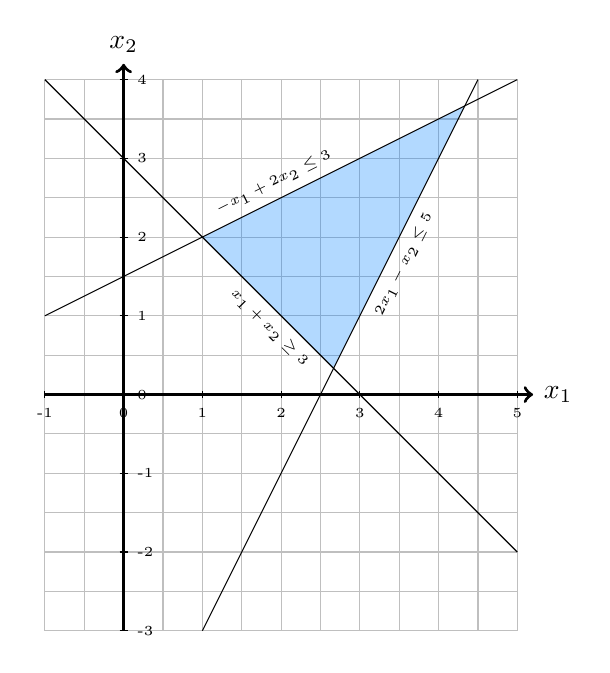
\begin{tikzpicture}
\draw[gray!50, thin, step=0.5] (-1,-3) grid (5,4);
\draw[very thick,->] (-1,0) -- (5.2,0) node[right] {$x_1$};
\draw[very thick,->] (0,-3) -- (0,4.2) node[above] {$x_2$};
%
\foreach \x in {-1,...,5} \draw (\x,0.05) -- (\x,-0.05) node[below] {\tiny\x};
\foreach \y in {-3,...,4} \draw (-0.05,\y) -- (0.05,\y) node[right] {\tiny\y};
%
\fill[blue!50!cyan,opacity=0.3] (8/3,1/3) -- (1,2) -- (13/3,11/3) -- cycle;
%
\draw (-1,4) -- node[below,sloped] {\tiny$x_1+x_2\geq3$} (5,-2);
\draw (1,-3) -- (3,1) -- node[below left,sloped] {\tiny$2x_1-x_2\leq5$} (4.5,4);
\draw (-1,1) -- node[above,sloped] {\tiny$-x_1+2x_2\leq3$} (5,4);
%
\end{tikzpicture}\footnote{%
\url{https://tex.stackexchange.com/questions/75933/how-to-draw-the-region-of-inequality}%
}
\caption{Feasible region of a generic linear program with constraints $x_1+x_2\geq 3$, $2x_1-x_2\leq 5$, and $-x_1+2x_2\leq 3$. The shaded triangle illustrates how three linear inequalities can carve out a bounded polygonal region.}
\label{fig:GenericThreeConstraintRegion}
\end{figure}
%
% Removed borrowed plot (replaced by recreated TikZ above) -- May 13, 2026
% Was: \begin{center}\altincludegraphics[width=0.8\linewidth]{images/lemon}{...} \end{center}
% Source: external-sources/lineqlpbook/images/lemon.{pdf,svg,fig} (Cheung, CC BY-SA 4.0).
% The lemon.pdf image showed the same Lemonade Vendor LP that is recreated in
% the TikZ figure above (Figure~\ref{fig:LemonadeVendorFeasibleRegion}).

In Figure~\ref{fig:LemonadeVendorFeasibleRegion}, level curves of \(z = 3x+2y\) are
drawn for several values of \(z\). From the picture, we can see that if \(z\) is greater than 6.8,
the line defined by \(3x+2y = z\) will not intersect the feasible
region. Hence, the profit cannot exceed 6.8 dollars.

As the line \(3x+2y = 6.8\) does intersect the feasible region, \(6.8\)
is the maximum value for the objective function. Note that there is only
one point in the feasible region that intersects the line \(3x+2y=6.8\),
namely $(x,y) = (1.2,1.6)$.
In other words, to maximize profit, we want to make 1.2 units of
lemonade and 1.6 units of lemon juice.
\end{solution}

The examples above each have a single optimal solution. However, four qualitatively different outcomes are possible for any linear program:
\begin{enumerate}[nosep]
\item A unique optimal solution (as we have already seen).
\item Infinitely many optimal solutions (the optimal level curve is parallel to an edge of the feasible region).
\item The problem is unbounded: the objective value can be made arbitrarily large (maximization) or small (minimization).
\item The problem is infeasible: no point satisfies all constraints simultaneously.
\end{enumerate}

The third outcome can only arise when the feasible region is unbounded. We will illustrate each of these outcomes below and, in a later chapter, prove that these are the only possibilities.

\section{Infinitely Many Optimal Solutions}\label{sec:infinitely-many-optima}

It is possible for a linear program to have more than one optimal solution. When this happens, there are in fact infinitely many.  We illustrate with a modification of the Furniture Workshop.

\begin{example}{Furniture Workshop: Alternative Objective}\label{exa:FurnitureWorkshopAltOpt}
Suppose the workshop in Example~\ref{ex:FurnitureWorkshop} revises its pricing so that each chair earns \$2 and each table earns \$1. The new objective function is $z(x_1,x_2) = 2x_1 + x_2$, while the constraints remain unchanged:
\begin{equation}
\begin{aligned}
\max\;\;& z(x_1,x_2) = 2x_1 + x_2\\
\text{s.t.}\;\;&  2x_1 + x_2 \leq 80\\
& x_1 + 3x_2 \leq 90\\
& x_1 \leq 35\\
& x_1, x_2 \geq 0
\end{aligned}
\label{eqn:FurnitureWorkshopAltOpt}
\end{equation}
\end{example}

\begin{solution}
The gradient of the new objective is $\nabla z = (2,1)$, which is parallel to the constraint $2x_1 + x_2 = 80$. As we sweep the level curves in the gradient direction, the last level curve that touches the feasible region coincides with the entire edge from $(30,20)$ to $(35,10)$.  Along this edge, $2x_1+x_2 = 80$ for every point, so $z = 80$ everywhere on it.

\begin{figure}[H]
\centering
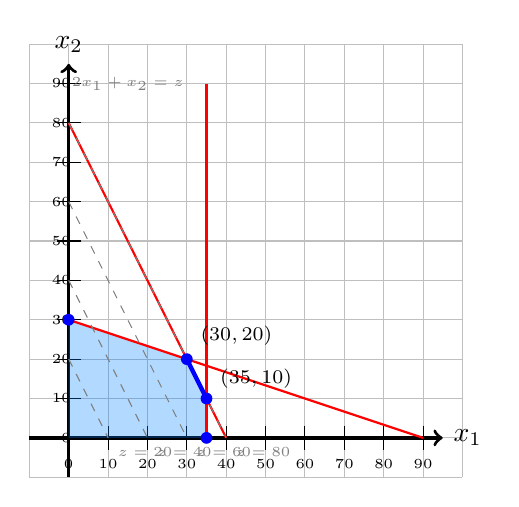
\begin{tikzpicture}[scale=0.05]
    % Grid and axes
    \draw[gray!50, thin, step=10] (-10,-10) grid (100,100);
    \draw[very thick,->] (-10,0) -- (95,0) node[right] {$x_1$};
    \draw[very thick,->] (0,-10) -- (0,95) node[above] {$x_2$};

    \foreach \x in {0,10,...,90} \draw (\x,3) -- (\x,-3) node[below] {\tiny\x};
    \foreach \y in {0,10,...,90} \draw (-3,\y) -- (3,\y) node[left] {\tiny\y};

    % Feasible region
    \fill[blue!50!cyan,opacity=0.3]
        (0,0) -- (0,30) -- (30,20) -- (35,10) -- (35,0) -- cycle;

    % Constraint lines
    \draw[red,thick] (0,80) -- (40,0);
    \draw[red,thick] (0,30) -- (90,0);
    \draw[red,thick] (35,90) -- (35,0);

    % Level curves (2x1 + x2 = z) slope = -2
    \draw[dashed,gray] (0,20) -- (10,0) node[below right] {\tiny $z = 20$};
    \draw[dashed,gray] (0,40) -- (20,0) node[below right] {\tiny $z = 40$};
    \draw[dashed,gray] (0,60) -- (30,0) node[below right] {\tiny $z = 60$};
    \draw[dashed,gray] (0,80) -- (40,0) node[below right] {\tiny $z = 80$};

    % Highlight the optimal edge
    \draw[blue,ultra thick] (30,20) -- (35,10);

    % Vertices
    \node[blue] at (0,30) [circle,fill,inner sep=1.5pt]{};
    \node[blue] at (30,20) [circle,fill,inner sep=1.5pt]{};
    \node[blue] at (35,10) [circle,fill,inner sep=1.5pt]{};
    \node[blue] at (35,0) [circle,fill,inner sep=1.5pt]{};

    \node[black,anchor=south west] at (31,21) {\scriptsize $(30,20)$};
    \node[black,anchor=south west] at (36,10) {\scriptsize $(35,10)$};

    \node[gray] at (15,90) {\tiny $2x_1 + x_2 = z$};
\end{tikzpicture}
\caption{Alternative optimal solutions: the level curve $z = 80$ (bold blue segment) lies along an entire edge of the feasible region. Every point on this edge is an optimal solution.}
\label{fig:FurnitureWorkshopAltOptSoln}
\end{figure}

Let $P$ denote the feasible region. For any $x_1^* \in [30,35]$ with $x_2^* = 80 - 2x_1^*$, the point $(x_1^*,x_2^*)$ lies on the edge from $(30,20)$ to $(35,10)$, and $z(x_1^*,x_2^*) = 80 \geq z(x_1,x_2)$ for all $(x_1,x_2)\in P$. Since there are infinitely many such points, the problem has infinitely many optimal solutions.
\label{ex:FurnitureWorkshopAltOptSoln}
\end{solution}

Based on this example, we extend our graphical algorithm to handle multiple optimal solutions:
\begin{stepbox}{algenter}{\ding{193}\ Graphical Method 2: Allowing Multiple Optima}
\emph{Everything from Method 1, plus a check for ties.}
\begin{enumerate}[nosep]
\item Sketch the feasible region by plotting each constraint boundary.
\item Draw level curves of the objective function for several values of $z$.
\item Sweep the level curves in the gradient direction to find the optimal value of $z$ that still intersects the feasible region. An optimal solution will occur at a vertex.
\item If the optimal level curve is parallel to an edge of the feasible region adjacent to the optimal vertex, then every point on that edge is also optimal. The problem has infinitely many optimal solutions.
\end{enumerate}
\end{stepbox}

\begin{learningcheckpoint}[label={lc:how-many-optima}]
Consider the graphical representation below.  How many optimal solutions are there if we are maximizing?  How about if we are minimizing?
\begin{center}
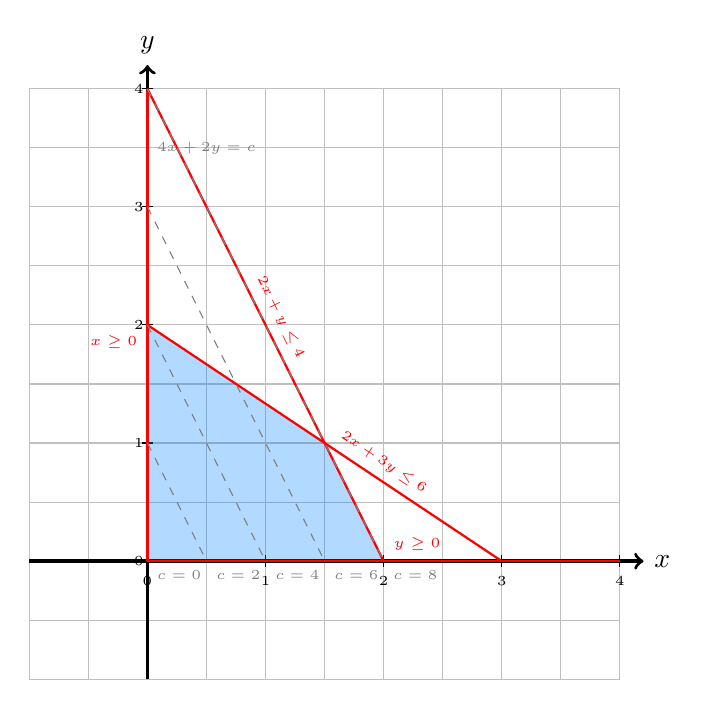
\begin{tikzpicture}[scale = 1.5]
    % Grid and axes
    \draw[gray!50, thin, step=0.5] (-1,-1) grid (4,4);
    \draw[very thick,->] (-1,0) -- (4.2,0) node[right] {$x$};
    \draw[very thick,->] (0,-1) -- (0,4.2) node[above] {$y$};

    % Axis labels
    \foreach \x in {0,...,4} \draw (\x,0.05) -- (\x,-0.05) node[below] {\tiny\x};
    \foreach \y in {0,...,4} \draw (-0.05,\y) -- (0.05,\y) node[left] {\tiny\y};

    % Shaded feasible region
    \fill[blue!50!cyan,opacity=0.3] (0,0) -- (0,2) -- (1.5,1) -- (2,0) -- cycle;

    % Constraint lines
    \draw[red,thick] (0,2) -- node[above right,sloped] {\tiny$2x + 3y \leq 6$} (3,0);
    \draw[red,thick] (0,4) -- node[above,sloped] {\tiny$2x + y \leq 4$} (2,0);
    \draw[red,thick] (0,0) -- node[below left] {\tiny$x \geq 0$} (0,4);
    \draw[red,thick] (0,0) -- node[above right] {\tiny$y \geq 0$} (4,0);

        % Objective function contours
            \draw[dashed,gray] (0,4) -- (2,0) node[below right] {\tiny$c=8$};
    \draw[dashed,gray] (0,3) -- (1.5,0) node[below right] {\tiny$c=6$};
    \draw[dashed,gray] (0,2) -- (1,0) node[below right] {\tiny$c=4$};
    \draw[dashed,gray] (0,1) -- (0.5,0) node[below right] {\tiny$c=2$};
    \draw[dashed,gray] (0,0) -- (0,0) node[below right] {\tiny$c=0$};

    % Contour labels
    \node[gray] at (0.5,3.5) {\tiny$4x + 2y = c$};

\end{tikzpicture}
\end{center}
\end{learningcheckpoint}

\section{Problems with No Solution}\label{sec:no-solution}

When the constraints of a linear program contradict one another, no point can satisfy them all. The feasible region is empty and we say the problem is \emph{infeasible}.

\begin{example}{Infeasible Problem}\label{exa:LPInfeasible}
 Consider the following linear programming problem:
\begin{equation}
\begin{aligned}
\max\;\;& z(x_1,x_2) = 4x_1 + 3x_2\\
\text{s.t.}\;\;& x_1 + x_2 \leq 8\\
& 2x_1 + x_2 \leq 12\\
& x_1 \geq 7\\
& x_2 \geq 5
\end{aligned}
\label{eqn:LPInfeasible}
\end{equation}
\end{example}
\begin{solution}
The constraints are plotted in Figure~\ref{fig:LPInfeasible}. The first two constraints restrict $x_1+x_2\leq 8$, but the lower bounds $x_1\geq 7$ and $x_2\geq 5$ together require $x_1+x_2\geq 12$. These are contradictory, so no point satisfies all constraints simultaneously.

\begin{figure}[H]
\centering
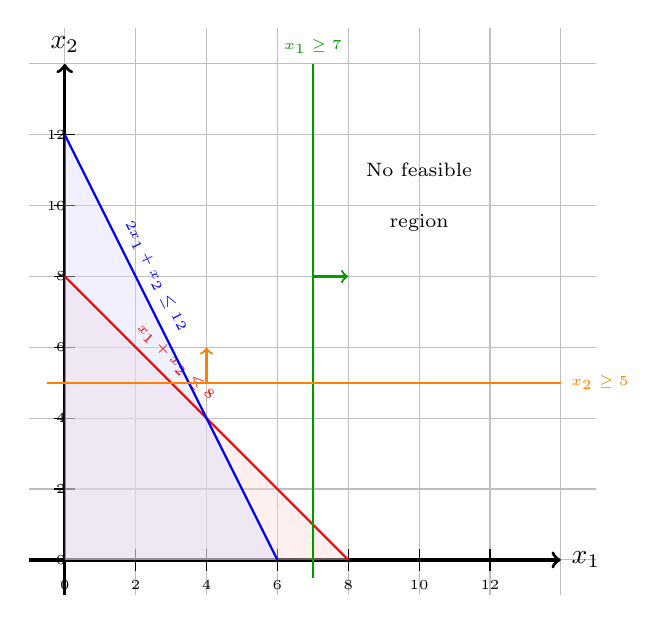
\begin{tikzpicture}[scale=0.45]
    % Grid and axes
    \draw[gray!50, thin, step=2] (-1,-1) grid (15,15);
    \draw[very thick,->] (-1,0) -- (14,0) node[right] {$x_1$};
    \draw[very thick,->] (0,-1) -- (0,14) node[above] {$x_2$};

    \foreach \x in {0,2,...,12} \draw (\x,0.3) -- (\x,-0.3) node[below] {\tiny\x};
    \foreach \y in {0,2,...,12} \draw (-0.3,\y) -- (0.3,\y) node[left] {\tiny\y};

    % Constraint regions
    \fill[red!15,opacity=0.4] (0,8) -- (8,0) -- (0,0) -- cycle;
    \fill[blue!15,opacity=0.4] (0,12) -- (6,0) -- (0,0) -- cycle;

    % Constraint lines
    \draw[red,thick] (0,8) -- node[above left, sloped] {\tiny $x_1 + x_2 \leq 8$} (8,0);
    \draw[blue,thick] (0,12) -- node[above left, sloped] {\tiny $2x_1 + x_2 \leq 12$} (6,0);
    \draw[green!60!black,thick] (7,-0.5) -- (7,14) node[above] {\tiny $x_1 \geq 7$};
    \draw[orange,thick] (-0.5,5) -- (14,5) node[right] {\tiny $x_2 \geq 5$};

    % Arrows showing required direction
    \draw[->,green!60!black,thick] (7,8) -- (8,8);
    \draw[->,orange,thick] (4,5) -- (4,6);

    % Infeasibility label
    \node[black] at (10,11) {\scriptsize No feasible};
    \node[black] at (10,9.5) {\scriptsize region};
\end{tikzpicture}
\caption{An infeasible linear program. The upper-bound constraints force $x_1+x_2\leq 8$, but the lower bounds require $x_1\geq 7$ and $x_2\geq 5$, so $x_1+x_2\geq 12$. No point can satisfy both conditions, and the feasible region is empty.}
\label{fig:LPInfeasible}
\end{figure}

Since the feasible region is empty, the problem has no solution.
\label{ex:LPNoSoln}
\end{solution}
Before stating the complete graphical algorithm, we also consider the case of unbounded feasible regions.

\section{Problems with Unbounded Feasible Regions}\label{sec:unbounded-regions}

Consider the problem

\begin{align*}
\min \quad && z = 5x_1 + 7x_2  \\
\text{s.t.} \quad && x_1 + 3x_2 &\geq 6 \\
&& 5x_1 + 2x_2 &\geq 10 \\
&& x_2 &\leq 4 \\
&& x_1, x_2 &\geq 0
\end{align*}

\begin{center}
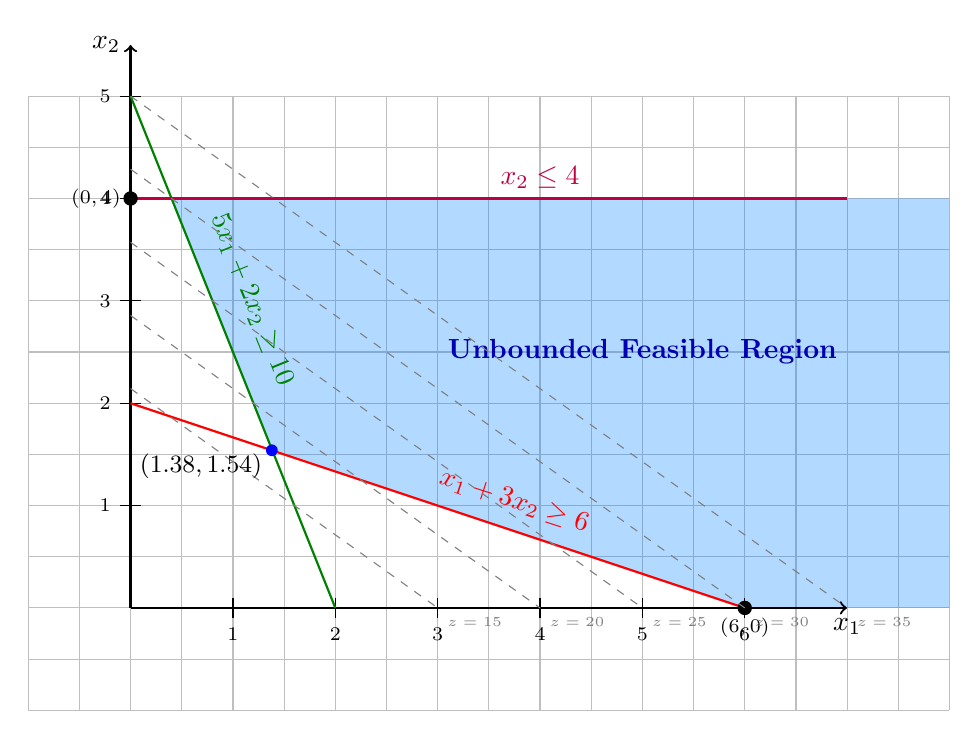
\begin{tikzpicture}[scale = 1.3]
    \draw[gray!50, thin, step=0.5] (-1,-1) grid (8,5);

    % Highlight the feasible region
    \fill[blue!50!cyan,opacity=0.3]
        (0.4,4) -- (1.39,1.55)  -- (6,0) -- (8,0) -- (8,4) -- cycle;

    % Define axes
    \draw[thick,->] (0,0) -- (7,0) node[anchor=north] {$x_1$};
    \draw[thick,->] (0,0) -- (0,5.5) node[anchor=east] {$x_2$};

    % Add tick marks on the x_1-axis
    \foreach \x in {1,2,3,4,5,6} {
        \draw (\x,0.1) -- (\x,-0.1) node[anchor=north] {\scriptsize $\x$};
    }

    % Add tick marks on the x_2-axis
    \foreach \y in {1,2,3,4,5} {
        \draw (0.1,\y) -- (-0.1,\y) node[anchor=east] {\scriptsize $\y$};
    }

    % Define the constraints
    % Line 1: X + 3Y = 6
    \draw[red,thick] (0,2) -- (6,0);
    \node[red, rotate=-18, anchor=north west] at (3,1.5) {$x_1 + 3x_2 \geq 6$};

    % Line 2: 5X + 2Y = 10
    \draw[green!50!black,thick] (0,5) -- (2,0);
    \node[green!50!black, rotate=-68, anchor=north west] at (1,4) {$5x_1 + 2x_2 \geq 10$};

    % Line 3: Y = 4
    \draw[purple,thick] (0,4) -- (7,4);
    \node[purple, rotate=0, anchor=south] at (4,4) {$x_2 \leq 4$};

    % Label feasible region
    \node[blue!70!black, font=\bfseries] at (5,2.5) {Unbounded Feasible Region};

    % Mark intersection points
\fill[black] (0,4) circle (2pt) node[anchor=east] {\scriptsize $(0,4)$};
\fill[black] (6,0) circle (2pt) node[anchor=north] {\scriptsize $(6,0)$};

% Objective function contours
\foreach \c in {15,20,25,30,35} {
    \draw[dashed,gray] (0,\c/7) -- (\c/5,0) node[below right] {\tiny$z = \c$};
    }
\node[blue,circle,fill,inner sep=1.5pt,label={[black,anchor=north east]\small$(1.38,1.54)$}] at (1.38,1.54) {};

\end{tikzpicture}
\end{center}

%% Original figure removed (file not available)

As you can see, the feasible region is \emph{unbounded}.  In particular, from any point in the feasible region, one can always find another feasible point by increasing the $x_1$ coordinate (i.e., move to the right in the picture).   However, this does not necessarily mean that the optimization problem is unbounded.

Indeed, the optimal solution is at $\mathbf{x}^* = (1.38, 1.54)$, the extreme point in the lower left hand corner,
with optimal objective value
$$
z^* = 5 \cdot 1.38 + 7\cdot 1.54 = 17.7.
$$

Consider however, if we consider a different problem where we try to maximize the objective
\begin{align*}
{\color{red} \max }\quad && z = 5x_1 + 7x_2  \\
\text{s.t.} \quad && x_1 + 3x_2 &\geq 6 \\
&& 5x_1 + 2x_2 &\geq 10 \\
&& x_2 &\leq 4 \\
&& x_1, x_2 &\geq 0
\end{align*}

\begin{solution}
This optimization problem is unbounded!  For example, notice that the point $(x_1,x_2) = (n,0)$ is feasible for all $n=1,2,3,\dots$.   Then the objective function $z = 5n + 0$ follows the sequence $5, 10, 15, \dots$, which diverges to infinity.
\end{solution}

We now illustrate two more scenarios with unbounded feasible regions. In the first, the problem is unbounded; in the second, a finite optimum exists despite the unbounded region.

\begin{example}{Unbounded Problem}\label{ex:LPUnboundFeasibleRegion1} Consider the linear programming problem:
\begin{equation}
\begin{aligned}
\max\;\;& z(x_1,x_2) = x_1 + 3x_2\\
\text{s.t.}\;\;& x_1 - x_2 \leq 3\\
& x_1 + 2x_2 \geq 4\\
&x_1,x_2 \geq 0
\end{aligned}
\label{eqn:LPUnboundFeasibleRegion1}
\end{equation}
\end{example}
\begin{solution}
The feasible region and level curves are shown in Figure~\ref{fig:LPUnboundFeasibleRegion1}.

\begin{figure}[H]
\centering
\begin{tikzpicture}[scale = 0.9]
    \draw[gray!50, thin, step=1] (-1,-1) grid (9,8);
    \draw[very thick,->] (-1,0) -- (9,0) node[right] {$x_1$};
    \draw[very thick,->] (0,-1) -- (0,8) node[above] {$x_2$};

    \foreach \x in {0,...,8} \draw (\x,0.05) -- (\x,-0.05) node[below] {\tiny\x};
    \foreach \y in {0,...,7} \draw (-0.05,\y) -- (0.05,\y) node[left] {\tiny\y};

    % Feasible region (unbounded upward-right)
    % Vertices: (0,2), (10/3, 1/3), then extends along both boundary lines
    \fill[blue!50!cyan,opacity=0.3] (0,2) -- (10/3,1/3) -- (9,6) -- (9,8) -- (0,8) -- cycle;

    % Constraint lines
    \draw[red,thick] (0,-3) -- node[below right,sloped,pos=0.7] {\tiny$x_1 - x_2 \leq 3$} (8,5);
    \draw[red,thick] (4,0) -- node[below left,sloped,pos=0.3] {\tiny$x_1 + 2x_2 \geq 4$} (0,2);
    \draw[red,thick] (0,0) -- node[below left] {\tiny$x_1 \geq 0$} (0,8);

    % Level curves (x1 + 3x2 = z)
    \draw[dashed,gray] (3,0) -- (0,1) node[left] {\tiny$z=3$};
    \draw[dashed,gray] (6,0) -- (0,2) node[left] {\tiny$z=6$};
    \draw[dashed,gray] (9,0) -- (0,3) node[left] {\tiny$z=9$};
    \draw[dashed,gray] (9,1) -- (0,4) node[left] {\tiny$z=12$};
    \draw[dashed,gray] (9,2) -- (0,5) node[left] {\tiny$z=15$};

    \node[gray] at (6,7) {\tiny$x_1 + 3x_2 = z$};

    % Vertices
    \node[blue] at (0,2) [circle,fill,inner sep=1.5pt]{};
    \node[blue] at (10/3,1/3) [circle,fill,inner sep=1.5pt]{};
    \node[black,anchor=south east] at (0,2) {\scriptsize$(0,2)$};
    \node[black,anchor=north west] at (10/3,1/3) {\scriptsize$(\tfrac{10}{3},\tfrac{1}{3})$};
\end{tikzpicture}
\caption{An unbounded linear program. The feasible region extends infinitely upward and to the right. Level curves of $z = x_1 + 3x_2$ continue to intersect the feasible region for arbitrarily large $z$, so the problem is unbounded.}
\label{fig:LPUnboundFeasibleRegion1}
\end{figure}

The feasible region extends infinitely upward and to the right. For any target value $z_0$, we can find a feasible point achieving $z \geq z_0$. For instance, take $(x_1,x_2) = (0,t)$ for $t\geq 2$: then $0-t = -t \leq 3$ and $0+2t = 2t\geq 4$, so the point is feasible, and $z = 3t$, which grows without bound. Hence the optimal value is $+\infty$ and the problem is unbounded.
\end{solution}

An unbounded feasible region does not always lead to an unbounded objective. The key is whether the gradient of the objective points into the unbounded direction or away from it.

\begin{example}{Finite Optimum with Unbounded Feasible Region}\label{exa:LPUnboundFiniteSoln}
Consider the same feasible region as in Example~\ref{ex:LPUnboundFeasibleRegion1} but with a new objective:
\begin{equation}
\begin{aligned}
\min\;\;& z(x_1,x_2) = 3x_1 + x_2\\
\text{s.t.}\;\;& x_1 - x_2 \leq 3\\
& x_1 + 2x_2 \geq 4\\
&x_1,x_2 \geq 0
\end{aligned}
\label{eqn:LPUnboundFiniteSoln}
\end{equation}
\end{example}
\begin{solution}
The feasible region is the same unbounded region as before. However, we are now \emph{minimizing}, and the gradient $(3,1)$ points to the right and slightly upward, precisely into the unbounded part of the feasible region. Moving opposite to the gradient (toward smaller $z$) takes us to the lower-left corner of the feasible region.

\begin{figure}[H]
\centering
\begin{tikzpicture}[scale = 0.9]
    \draw[gray!50, thin, step=1] (-1,-1) grid (9,8);
    \draw[very thick,->] (-1,0) -- (9,0) node[right] {$x_1$};
    \draw[very thick,->] (0,-1) -- (0,8) node[above] {$x_2$};

    \foreach \x in {0,...,8} \draw (\x,0.05) -- (\x,-0.05) node[below] {\tiny\x};
    \foreach \y in {0,...,7} \draw (-0.05,\y) -- (0.05,\y) node[left] {\tiny\y};

    % Feasible region
    \fill[blue!50!cyan,opacity=0.3] (0,2) -- (10/3,1/3) -- (9,6) -- (9,8) -- (0,8) -- cycle;

    % Constraint lines
    \draw[red,thick] (0,-3) -- (8,5);
    \draw[red,thick] (4,0) -- (0,2);
    \draw[red,thick] (0,0) -- (0,8);

    % Level curves (3x1 + x2 = z)
    \draw[dashed,gray] (0,2) -- (2/3,0) node[below] {\tiny$z=2$};
    \draw[dashed,gray] (0,4) -- (4/3,0) node[below] {\tiny$z=4$};
    \draw[dashed,gray] (0,6) -- (2,0) node[below] {\tiny$z=6$};
    \draw[dashed,gray] (0,8) -- (8/3,0) node[below] {\tiny$z=8$};

    \node[gray] at (5,7) {\tiny$3x_1 + x_2 = z$};

    % Optimal vertex
    \node[blue] at (0,2) [circle,fill,inner sep=2pt]{};
    \node[black,anchor=south east] at (-0.2,2) {\scriptsize$(0,2)$};
    \node[blue] at (10/3,1/3) [circle,fill,inner sep=1.5pt]{};
    \node[black,anchor=north west] at (10/3,1/3) {\scriptsize$(\tfrac{10}{3},\tfrac{1}{3})$};
\end{tikzpicture}
\caption{A linear program with an unbounded feasible region but a finite optimal solution. The minimum of $z = 3x_1+x_2$ occurs at the vertex $(0,2)$ with $z^* = 2$, because the gradient points away from the bounded end of the feasible region.}
\label{fig:LPUnboundFeasibleRegion2}
\end{figure}

Evaluating the objective at the vertices: $z(0,2) = 2$ and $z(\tfrac{10}{3},\tfrac{1}{3}) = 10 + \tfrac{1}{3} = \tfrac{31}{3} \approx 10.3$. Since we are minimizing, the optimum is $z^* = 2$ at $(x_1^*,x_2^*) = (0,2)$. Once again, the optimal solution occurs at a vertex of the feasible region, even though the region is unbounded.
\label{ex:LPUnboundFeasibleRegion2}
\end{solution}

We can now state a complete algorithm for graphically solving any two-variable linear program.

\begin{stepbox}{algopt}{\ding{51}\ The Complete Graphical Method for Two-Variable LPs}
\emph{Handles every case: infeasible, unbounded, unique, and multiple optima.}
\begin{enumerate}
    \item Sketch the feasible region by plotting the constraint boundaries and shading their intersection.
    \item If the feasible region is empty, the problem is \textbf{infeasible}; stop.
    \item Draw level curves of the objective function and determine the gradient direction.
    \item \textbf{Bounded feasible region:}
    \begin{enumerate}
        \item Sweep the level curves in the gradient direction (for maximization) or opposite (for minimization) to find the last level curve touching the feasible region. The optimal solution is at a vertex.
        \item If this optimal level curve is parallel to an edge of the feasible region, every point on that edge is optimal (infinitely many solutions).
    \end{enumerate}
    \item \textbf{Unbounded feasible region:}
    \begin{enumerate}
        \item If the level curves can be swept indefinitely while still intersecting the feasible region, the problem is \textbf{unbounded}.
        \item Otherwise, a finite optimum exists at a vertex; proceed as in the bounded case.
    \end{enumerate}
\end{enumerate}
\end{stepbox}

\newpage

\section{Exercises}\label{exercises}
\addcontentsline{toc}{section}{Exercises}

\exgroup{Warm-ups}

\begin{ex}{Feasible Region Analysis}{}
\stars{1}Consider the following system of constraints:
\[
x + y \geq 5
\]
\[
x \geq 0, \quad y \geq 0
\]
Which of the following statements is true about the feasible region?
\begin{enumerate}
    \item  The feasible region is a bounded polygon.
    \item The feasible region is an unbounded region.
    \item The feasible region consists of a single point.
    \item The problem is infeasible.
\end{enumerate}
\exrefs{\S\ref{sec:nonempty-bounded}, \S\ref{sec:unbounded-regions}}
\end{ex}

\begin{ex}{Sketch Feasible Region}{}\label{ex:feasible-region}
\stars{1}Sketch all \(\begin{bmatrix} x \\ y \end{bmatrix}\) satisfying
\[
x - 2y \leq 2
\]
on the \((x,y)\)-plane.
\exrefs{\S\ref{sec:nonempty-bounded}}
\end{ex}

\begin{ex}{Graphical Method 1 Practice}{}\label{ex:graphical-method-one}
\stars{1}Apply the steps of the box ``Graphical Method 1: Bounded Region, Unique Optimum'' to the linear program
\begin{align*}
\max \quad & 3x + 2y\\
\text{s.t.} \quad & x + y \leq 4\\
& x \leq 3\\
& x, y \geq 0.
\end{align*}
Sketch the feasible region, list all four vertices, and sweep the level curves of $z = 3x + 2y$ in the gradient direction to find the optimal solution and the optimal value.
\exrefs{\S\ref{sec:graphical-approach}, Example~\ref{ex:FurnitureWorkshop}}
\end{ex}

\begin{ex}{Graphical Method for Lemonade Vendor}{}
\stars{1}Solve the Lemonade Vendor problem from Example~\ref{exa:lemonadevendor} using the graphical method.
\exrefs{\S\ref{sec:graphical-approach}, Example~\ref{exa:lemonadevendor}}
\end{ex}

\exgroup{Core problems}

\begin{ex}{Graphical Method}{}
\stars{2}Use the graphical method to determine two optimal solutions to linear program:
\begin{align*}
\min  \quad& 3x_1 + 5x_2\\
 & 3x_1 + 2x_2 \ge 36\\
 & 6x_1 + 10x_2 \geq 90\\
 & x_1, x_2 \geq 0
\end{align*}
\exrefs{\S\ref{sec:infinitely-many-optima}, Example~\ref{exa:FurnitureWorkshopAltOpt}}
\end{ex}

\begin{ex}{Infeasible Region Graph}{}\label{ex:infeasible}
\stars{2}Graph the feasible region of the linear program:
\begin{align*}
\min  \quad & x_1 - x_2\\
 & x_1 + x_2 \leq 6\\
 & x_1 - x_2 \geq 1\\
 & x_2 - x_1 \geq 3\\
 & x_1, x_2 \geq 0
\end{align*}
Without considering the objective function, how many feasible solutions are there?  Justify your answer.
\exrefs{\S\ref{sec:no-solution}, Example~\ref{exa:LPInfeasible}}
\end{ex}

\begin{ex}{Determine Optimal Value}{}\label{ex:lp-optimal-value}
\stars{2}Determine the optimal value of
\[
\begin{array}{rl}
\text{Minimize} & x + y \\
\text{Subject to} &  2x + y \geq 4 \\
& x + 3y \geq 1.
\end{array}
\]
\exrefs{\S\ref{sec:graphical-approach}}
\end{ex}

\begin{ex}{Show Unbounded Problem}{}\label{ex:lp-unbounded}
\stars{2}Show that the problem
\[
\begin{array}{rl}
\text{Minimize} & -x + y \\
\text{Subject to} &  2x - y \geq 0 \\
& x + 3y \geq 3
\end{array}
\]
is unbounded.
\exrefs{\S\ref{sec:unbounded-regions}, Example~\ref{ex:LPUnboundFeasibleRegion1}}
\end{ex}

\begin{ex}{Bounded Solution on Unbounded Region}{}\label{exer:BoundedSolutionQuestion}
\stars{2}Consider the feasible region from Example~\ref{ex:LPUnboundFeasibleRegion1} (with $x_1-x_2\leq 3$ and $x_1+2x_2\geq 4$). Does the problem $\max\; z = -2x_1 + x_2$ subject to these constraints have a finite solution? Justify your answer using the Complete Graphical Method.
\exrefs{\S\ref{sec:unbounded-regions}, Example~\ref{exa:LPUnboundFiniteSoln}}
\end{ex}

\begin{ex}{Diet Problem}{}\label{ex:lp-diet-problem}
\stars{2}Suppose that you are shopping for dietary supplements to satisfy your
required daily intake of 0.40mg of nutrient \(M\) and 0.30mg of
nutrient \(N\). There are three popular products on the market. The
costs and the amounts of the two nutrients are given in the following
table:

\begin{table}[h!]
\centering
\begin{tabular}{lccc}
\toprule
         & Product 1 & Product 2 & Product 3 \\ \midrule
Cost     & \$27      & \$31      & \$24      \\
Daily amount of \(M\) & 0.16 mg   & 0.21 mg   & 0.11 mg   \\
Daily amount of \(N\) & 0.19 mg   & 0.13 mg   & 0.15 mg   \\ \bottomrule
\end{tabular}
\caption{Data for problem.}
\label{tab:your_table_label}
\end{table}

You want to determine how much of each product you should buy so that
the daily intake requirements of the two nutrients are satisfied at
minimum cost. Formulate your problem as a linear programming problem,
assuming that you can buy a fractional number of each product.
\exrefs{\S\ref{sec:graphical-approach}, Example~\ref{exa:lemonadevendor}}
\end{ex}

\exgroup{Concepts and connections}

\begin{ex}{Why Must an Optimum Be at a Vertex?}{}\label{ex:why-vertex}
\stars{2}Suppose a linear program in two variables has a nonempty and bounded feasible region.
\begin{enumerate}
\item Theorem~\ref{thm:optimalextremepoint} guarantees that some optimal solution occurs at a vertex. Explain why, using the level-curve picture: if a feasible point lies strictly inside the region, or strictly inside an edge, why can we always find a vertex whose objective value is at least as good?
\item Which part of your argument uses the assumption that the region is bounded? Give an example of an unbounded feasible region and an objective function for which no optimal solution exists at all.
\end{enumerate}
\exrefs{\S\ref{sec:nonempty-bounded}, Theorem~\ref{thm:optimalextremepoint}}
\end{ex}

\begin{ex}{Infinite Optimal Solutions}{}
\stars{2}Find an objective function for the feasible region in Example~\ref{ex:LPUnboundFeasibleRegion1} that produces infinitely many optimal solutions. Describe the set of optima.
\exrefs{\S\ref{sec:infinitely-many-optima}}
\end{ex}

\begin{ex}{Infinitely Many Optimal Solutions}{}
\stars{2}Modify the objective function in Example~\ref{exa:lemonadevendor} so that the resulting LP has infinitely many optimal solutions. Describe the complete set of optimal solutions.
\exrefs{\S\ref{sec:infinitely-many-optima}, Example~\ref{exa:lemonadevendor}}
\end{ex}

\begin{ex}{Bounded Optimum on Unbounded Region}{}
\stars{2}Consider the constraints $-x_1+x_2\leq 5$, $x_1+x_2\geq 2$, $x_1,x_2\geq 0$. Construct a \textbf{maximization} objective that has a finite optimum despite the unbounded feasible region. Sketch the feasible region and level curves to verify.

\emph{[Hint: Choose a gradient that points away from the unbounded direction.]}
\exrefs{\S\ref{sec:unbounded-regions}, Example~\ref{exa:LPUnboundFiniteSoln}}
\end{ex}

\exgroup{Challenge problems}

\begin{ex}{Unbounded Objective Direction}{}
\stars{3}Consider the following problem:
\[
\begin{array}{rrcrll}
\text{minimize } & -2x_1 & + & x_2 & \\
\text{subject to} & -x_1 & + & x_2 & \leq & 3 \\
& x_1 & - & 2x_2 & \leq & 2 \\
& x_1 & & & \geq & 0 \\
& & & x_2 & \geq & 0. \\
\end{array}
\]

\begin{enumerate}
\item Show that for any \(t \geq 0\),
\[
\begin{bmatrix} x_1 \\ x_2 \end{bmatrix} = \begin{bmatrix} t \\ t \end{bmatrix}
\]
satisfies all the constraints. Show that the objective function is unbounded for this point as $t \to \infty$.

\item Show that \[
\begin{bmatrix} x_1 \\ x_2 \end{bmatrix} = \begin{bmatrix} 2t+2 \\ t \end{bmatrix}
\]
 is feasible for any \(t \geq 0\).  What is the objective function value at this point?  Show that the objective function is unbounded (yet again) by letting $t \to \infty$.
 \end{enumerate}
\exrefs{\S\ref{sec:unbounded-regions}, Example~\ref{ex:LPUnboundFeasibleRegion1}}
 \end{ex}

\begin{ex}{Bounded and Unbounded Optimization}{}
\stars{3}Consider the following problem:

\[
\begin{array}{rrcllll}
\text{maximize/minimize } & 2x & + & 2y \\
\text{subject to} & -x & + & 2y & \leq & 12 \\
& 2x & + & y & \geq & 4 \\
& x & + & 2y & \geq & 5 \\
& x & & & \geq & 0 \\
& & & y & \geq & 0. \\
\end{array}
\]

\begin{enumerate}

\item Determine the minimum value of \(2x + 2y\) by solving (graphically) the corresponding optimization problem. Show that the minimum is attained at a bounded feasible point.

\item Show that the maximum value of \(2x + 2y\) is unbounded by finding a feasible solution of the form
\[
\begin{bmatrix} x \\ y \end{bmatrix} = \begin{bmatrix} 5\\ 0\end{bmatrix} + t \begin{bmatrix} 1\\ 0\end{bmatrix}
\]
for any \(t \geq 0\). Show that as \(t \to \infty\), the objective function becomes unbounded.

\item Show that
\[
\begin{bmatrix} x \\ y \end{bmatrix} = \begin{bmatrix} 0 \\ 6 \end{bmatrix} + t\begin{bmatrix} 2 \\ 1 \end{bmatrix}
\]
is feasible for any \(t \geq 0\). Compute the objective function value at this point and demonstrate that it is unbounded as \(t \to \infty\).

\end{enumerate}
\exrefs{\S\ref{sec:unbounded-regions}}
\end{ex}

\begin{ex}{From an Optimal Edge to a Unique Optimum}{}\label{ex:edge-of-optima}
\stars{3}Construct a tie between optimal solutions, then break it.
\begin{enumerate}
\item Construct a linear program in two variables whose set of optimal solutions is an entire edge of the feasible region, not just a single vertex. Sketch the feasible region, identify the optimal edge, and use the tie-checking step of Graphical Method 2 to explain why every point of that edge is optimal.
\item Now change exactly one coefficient in your objective function so that the modified LP has a unique optimal solution at a vertex of the same feasible region. Identify the new optimal vertex and explain why the tie disappears.
\end{enumerate}
\exrefs{\S\ref{sec:infinitely-many-optima}, Example~\ref{exa:FurnitureWorkshopAltOpt}}
\end{ex}

%By Kevin Cheung
%The book is licensed under the
%\href{http://creativecommons.org/licenses/by-sa/4.0/}{Creative Commons
%Attribution-ShareAlike 4.0 International License}.
%
%This file has been modified by Robert Hildebrand 2020.
%CC BY SA 4.0 licence still applies.

% Legacy fragment, fully commented 2026-07-08
%\section{Graphical example}\label{graphic}
%
%To motivate the subject of linear programming (LP), we begin with a
%planning problem that can be solved graphically.
%
%
%
%The above solution method can hardly be regarded as rigorous because we
%relied on a picture to conclude that \(3x + 2y \leq 6.8\) for all
%$(x,y)$ satisfying the constraints. But we
%can actually show this \emph{algebraically}.
%
%Note that multiplying both sides of the constraint \(x + 3y \leq 6\)
%gives \(0.2x + 0.6 y \leq 1.2\), and multiplying both sides of the
%constraint \(2x + y \leq 4\) gives \(2.8x + 1.4 y \leq 5.6\). Hence, any
%\(\begin{bmatrix} x\\y\end{bmatrix}\) that satisfies both \(x+3y\leq 6\)
%and \(2x+y \leq 4\) must also satisfy
%\((0.2x+0.6y) + (2.8x+1.4y) \leq 1.2 + 5.6\), which simplifies to
%\(3x + 2y \leq 6.8\) as desired! (Here, we used the fact that if
%\(a \leq b\) and \(c \leq d\), then \(a+c \leq b+d\).)
%
%Now, one might ask if it is always possible to find an algebraic proof
%like the one above for similar problems. If the answer is yes, how does
%one find such a proof? We will see answers to this question later on.
%
%Before we end this segment, let us consider the following problem:
%\[\begin{array}{rrcrll}
%\text{minimize } & -2x & + & y & \\
%\text{subject to} & -x & + & y & \leq & 3 \\
%& x & - &  2y & \leq & 2 \\
%& x &  & & \geq & 0 \\
%& & & y & \geq & 0. \\
%\end{array}\]
%
%Note that for any \(t \geq 0\),
%\(\begin{bmatrix} x \\ y\end{bmatrix} = \begin{bmatrix} t \\ t\end{bmatrix}\)
%satisfies all the constraints. The value of the objective function at
%\(\begin{bmatrix} x \\ y\end{bmatrix} = \begin{bmatrix} t \\ t\end{bmatrix}\)
%is \(-t\). As \(t \rightarrow \infty\), the value of the objective
%function tends to \(-\infty\). Therefore, there is no minimum value for
%the objective function. The problem is said to be unbounded. Later on,
%we will see how to detect unboundedness algorithmically.
%
%As an exercise, check that unboundedness can also be established by
%using
%\(\begin{bmatrix} x \\ y\end{bmatrix} = \begin{bmatrix} 2t+2 \\ t\end{bmatrix}\)
%for \(t \geq 0\).



\subsubsection*{Selected Solutions}
\label{solutions}
\addcontentsline{toc}{subsection}{Solutions}

\begin{solution}(Exercise~\ref{ex:graphical-method-one})
The feasible region has vertices $(0,0)$, $(3,0)$, $(3,1)$, and $(0,4)$. Evaluating the objective: $z(0,0)=0$, $z(3,0)=9$, $z(3,1)=11$, and $z(0,4)=8$. Sweeping the level curves of $z = 3x+2y$ in the direction of the gradient $(3,2)$, the last level curve to touch the region passes through $(3,1)$, where the constraints $x+y\leq 4$ and $x\leq 3$ are both binding. The optimal solution is $(x^*,y^*) = (3,1)$ with optimal value $z^* = 11$.
\end{solution}

\begin{solution}(Exercise~\ref{ex:infeasible})
In fact, constraints 2 and 3 point away from each other, and hence there are no feasible solutions.
\end{solution}

\begin{solution}(Exercise \ref{ex:feasible-region})

The points \((x,y)\) satisfying \(x-2y \leq 2\) are precisely those
above the line passing through \((2,0)\) and \((0,-1)\).
\end{solution}

\begin{solution}(\ref{ex:lp-optimal-value})

We want to determine the minimum value \(z\) so that \(x+y=z\) defines
a line that has a nonempty intersection with the feasible region.
However, we can avoid referring to a sketch by setting \(x=z-y\) and
substituting for \(x\) in the inequalities to obtain:

\begin{eqnarray*}
2(z-y) + y \geq 4 \\
(z-y) + 3y \geq 1,
\end{eqnarray*}

or equivalently,

\begin{eqnarray*}
z \geq 2+\frac{1}{2}y \\
z \geq 1-2y,
\end{eqnarray*}

Thus, the minimum value for \(z\) is
\(\min \{ 2+\frac{1}{2}y, 1-2y\}\), which occurs at
\(y = -\frac{2}{5}\). Hence, the optimal value is \(\frac{9}{5}\).

We can verify our work by doing the following. If our calculations
above are correct, then an optimal solution is given by
\(x = \frac{11}{5}\), \(y = -\frac{2}{5}\) since \(x = z - y\). It is
easy to check that this satisfies both inequalities and therefore is a
feasible solution.

Now, taking \(\frac{2}{5}\) times the first inequality and
\(\frac{1}{5}\) times the second inequality, we can infer the
inequality \(x+y \geq \frac{9}{5}\). The left-hand side of this
inequality is precisely the objective function. Hence, no feasible
solution can have objective function value less than \(\frac{9}{5}\).
But \(x = \frac{11}{5}\), \(y = -\frac{2}{5}\) is a feasible solution
with objective function value equal to \(\frac{9}{5}\). As a result,
it must be an optimal solution.

\textbf{Remark.} We have not yet discussed how to obtain the
multipliers \(\frac{2}{5}\) and \(\frac{1}{5}\) for inferring the
inequality \(x+y \geq \frac{9}{5}\). This is an issue that will be
taken up later. In the meantime, think about how one could have
obtained these multipliers for this particular exercise.
\end{solution}

\begin{solution}(Exercise \ref{ex:lp-unbounded})
We could glean some insight by first making a sketch on the
\((x,y)\)-plane.

The line defined by \(-x + y = z\) has \(x\)-intercept \(-z\). Note
that for \(z \leq -3\),
\(\begin{bmatrix} x\\y \end{bmatrix} = \begin{bmatrix} -z\\ 0\end{bmatrix}\)
satisfies both inequalities and the value of the objective function at
\(\begin{bmatrix} x\\y \end{bmatrix} = \begin{bmatrix} -z\\ 0\end{bmatrix}\)
is \(z\). Hence, there is no lower bound on the value of the objective
function.
\end{solution}

\begin{solution}(Exercise \ref{ex:lp-diet-problem})
Let \(x_i\) denote the amount of Product \(i\) to buy for
\(i = 1,2,3\). Then, the problem can be formulated as
\[
\begin{array}{rrcrcrll}
\text{minimize } & 27 x_1 & + & 31 x_2 & + & 24 x_3 \\
\text{subject to}
& 0.16 x_1 & + & 0.21 x_2 & + & 0.11 x_3 & \geq & 0.40 \\
& 0.19 x_1 & + & 0.13 x_2 & + & 0.15 x_3 & \geq & 0.30 \\
& x_1 & , & x_2 & , & x_3 & \geq & 0. \\
\end{array}
\]

\textbf{Remark.} If one cannot buy fractional amounts of the products,
the problem can be formulated as
\[
\begin{array}{rrcrcrll}
\text{minimize } & 27 x_1 & + & 31 x_2 & + & 24 x_3 \\
\text{subject to}
& 0.16 x_1 & + & 0.21 x_2 & + & 0.11 x_3 & \geq & 0.40 \\
& 0.19 x_1 & + & 0.13 x_2 & + & 0.15 x_3 & \geq & 0.30 \\
& x_1 & , & x_2 & , & x_3 & \geq & 0. \\
& x_1 & , & x_2 & , & x_3 & \in & \mathbb{Z}. \\
\end{array}
\]
\end{solution}

\section{Extreme Directions}

We now define a procedure for finding the extreme directions, using the following LP's feasible region.  Graphically, we can see that the extreme directions should follow the $s_1=0$ (red) line and the $s_3 = 0$ (orange) line.

\begin{minipage}[t][][b]{.4\linewidth}
\begin{align*}
\max \quad & z = -5x_1 - x_2  \\
\text{s.t.} \quad & x_1 - 4x_2 +s_1 = 0  \\
& -x_1 + x_2 + s_2 = 1 \\
& -x_1 + 2x_2 +s_3 = 4 \\
& x_1, x_2, s_1, s_2, s_3 \ge 0.
\end{align*}
\end{minipage}%
\begin{minipage}[t][][b]{.6\linewidth}
\begin{center}  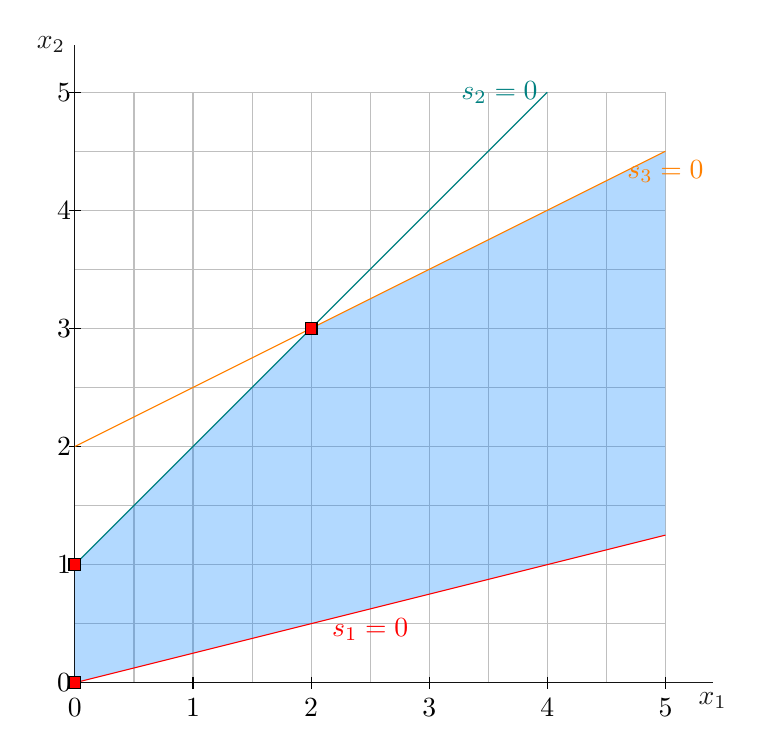
\begin{tikzpicture} [scale=1.5]
    \draw[gray!50, thin, step=.5] (0,0) grid (5,5);
    \draw[opacity=0.9] (0,0) -- (5.4,0) node[below] {$x_1$};
    \draw[opacity=0.9] (0,0) -- (0,5.4) node[left] {$x_2$}; % option \draw[very thick,->]

    \foreach \x in {0,...,5} \draw (\x,0.05) -- (\x,-0.05) node[below] {\x};
    \foreach \y in {0,...,5} \draw (-0.05,\y) -- (0.05,\y) node[left] {\y};

    \fill[blue!50!cyan,opacity=0.3] (0,0) -- (0,1) -- (2,3) -- (5,4.5) --(5,1.25)-- cycle;

    \draw [red](0,0) -- node[below] {$s_1=0$} (5, 1.25);
    \draw [teal] (0,1)  --  (4,5) node[left, sloped] {$s_2=0$};
    \draw [orange](0,2) --  (5,4.5) node[below, sloped] {$s_3=0$}; %node[above right ,sloped]

    \node[fill=blue,circle,inner sep=0.05cm] at (0,0) {};
\node[fill=blue,circle,inner sep=0.05cm] at (0,1) {};
\node[fill=blue,circle,inner sep=0.05cm] at (2,3) {};

\filldraw[fill=red] (-0.05,-0.05) rectangle (0.05,0.05);
\filldraw[fill=red] (-0.05,.95) rectangle (0.05,1.05);
\filldraw[fill=red] (1.95,2.95) rectangle (2.05,3.05);
\end{tikzpicture} \end{center}
\end{minipage}

\begin{center}  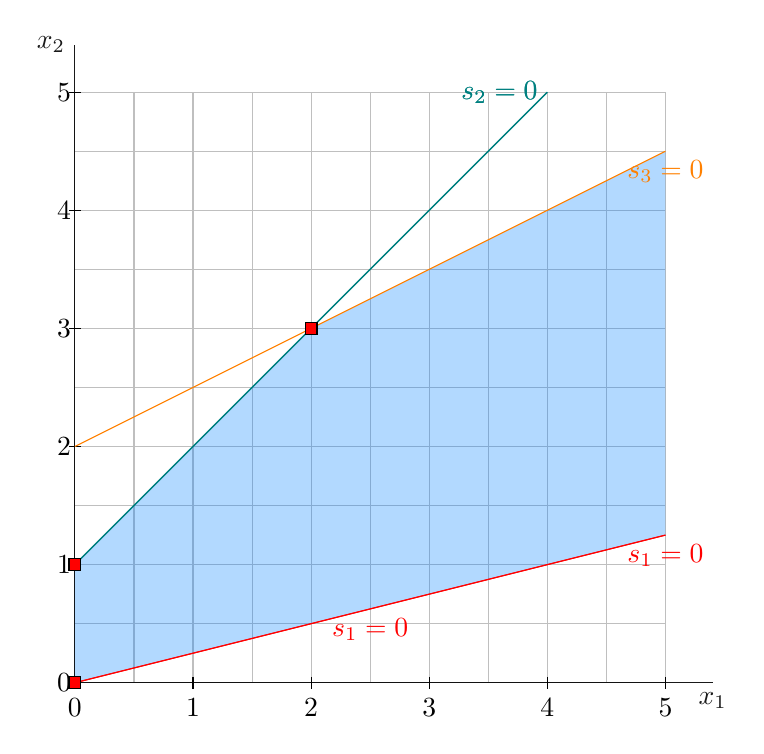
\begin{tikzpicture} [scale=1.5]
    \draw[gray!50, thin, step=.5] (0,0) grid (5,5);
    \draw[opacity=0.9] (0,0) -- (5.4,0) node[below] {$x_1$};
    \draw[opacity=0.9] (0,0) -- (0,5.4) node[left] {$x_2$}; % option \draw[very thick,->]

    \foreach \x in {0,...,5} \draw (\x,0.05) -- (\x,-0.05) node[below] {\x};
    \foreach \y in {0,...,5} \draw (-0.05,\y) -- (0.05,\y) node[left] {\y};

    \fill[blue!50!cyan,opacity=0.3] (0,0) -- (0,1) -- (2,3) -- (5,4.5) --(5,1.25)-- cycle;

\draw[domain=0:4,smooth,variable=\x, teal] plot ({\x},{\x+1}) node[left] {$s_2=0$};
\draw[domain=0:5,smooth,variable=\x, red] plot ({\x},{\x*1/4}) node[below] {$s_1=0$};
\draw [red](0,0) -- node[below] {$s_1=0$} (5, 1.25);
    \draw [teal] (0,1)  --  (4,5) node[left, sloped] {$s_2=0$};
    \draw [orange](0,2) --  (5,4.5) node[below, sloped] {$s_3=0$}; %node[above right ,sloped]
    \node[fill=blue,circle,inner sep=0.05cm] at (0,0) {};
\node[fill=blue,circle,inner sep=0.05cm] at (0,1) {};
\node[fill=blue,circle,inner sep=0.05cm] at (2,3) {};

\filldraw[fill=red] (-0.05,-0.05) rectangle (0.05,0.05);
\filldraw[fill=red] (-0.05,.95) rectangle (0.05,1.05);
\filldraw[fill=red] (1.95,2.95) rectangle (2.05,3.05);
\end{tikzpicture} \end{center}

%\draw[scale=0.5,domain=-3:3,smooth,variable=\x,blue] plot ({\x},{\x*\x}); % commented out - was outside tikzpicture

\medskip E.g., consider the $s_3=0$ (orange) line, to find the extreme direction start at extreme point (2,3) and find another feasible point on the orange line, say (4,4) and subtract (2,3) from (4,4), which yields (2,1).

\medskip This is related to the slope in two dimensions: the rise is 1 and the run is 2. So this direction has a slope of 1/2, but this does not carry over easily to higher dimensions where directions cannot be defined by a single number.

\medskip To find the extreme directions we can change the right-hand-side to $\mathbf{b} = \mathbf{0}$, which forms a polyhedral cone (in yellow), and then add the constraint $x_1 + x_2 = 1$. The intersection of the cone and  $x_1 + x_2 = 1$ form a line segment.

\begin{minipage}[t][][b]{.4\linewidth} \vspace{0mm}
\begin{align*}
\max \quad & z = -5x_1 - x_2  \\
\text{s.t.} \quad & x_1 - 4x_2 +s_1 = 0  \\
& -x_1 + x_2 + s_2 = 0 \\
& -x_1 + 2x_2 +s_3 = 0 \\
& x_1 + x_2 = 1 \\
& x_1, x_2, s_1, s_2, s_3 \ge 0.
\end{align*}
\end{minipage}%
\begin{minipage}[t][][b]{.6\linewidth}
\begin{center} 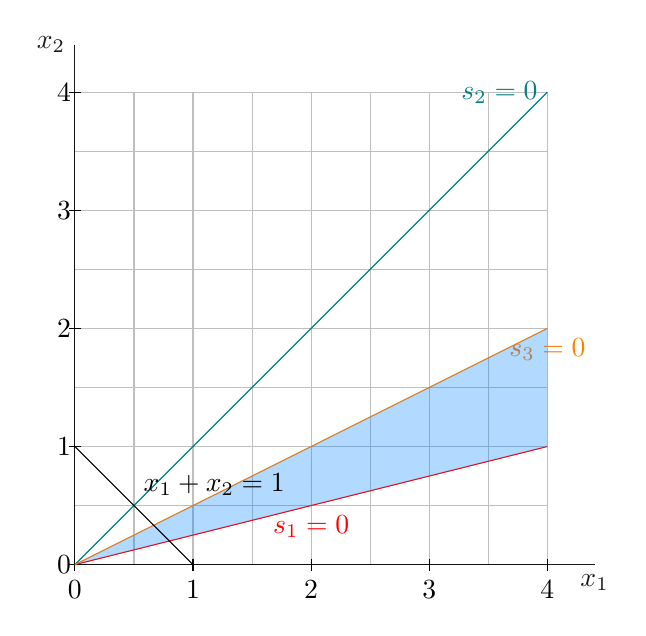
\begin{tikzpicture} [scale=1.5]
\draw[gray!50, thin, step=.5] (0,0) grid (4,4);
\draw[opacity=0.9] (0,0) -- (4.4,0) node[below] {$x_1$};
\draw[opacity=0.9] (0,0) -- (0,4.4) node[left] {$x_2$}; % option \draw[very thick,->]

\foreach \x in {0,...,4} \draw (\x,0.05) -- (\x,-0.05) node[below] {\x};
\foreach \y in {0,...,4} \draw (-0.05,\y) -- (0.05,\y) node[left] {\y};

\draw [red](0, 0) -- node[below] {$s_1=0$} (4, 1);
\draw [teal] (0,0)  -- (4,4) node[left, sloped] {$s_2=0$};
\draw [orange](0,0) -- (4,2) node[below, sloped] {$s_3=0$};
\fill[blue!50!cyan,opacity=0.3] (0,0) -- (4,2) -- (4,1) --  cycle;

\draw [black] (0,1)  -- node[above right] {$x_1+x_2 = 1$} (1,0);
\end{tikzpicture} \end{center}
\end{minipage}

\begin{center} 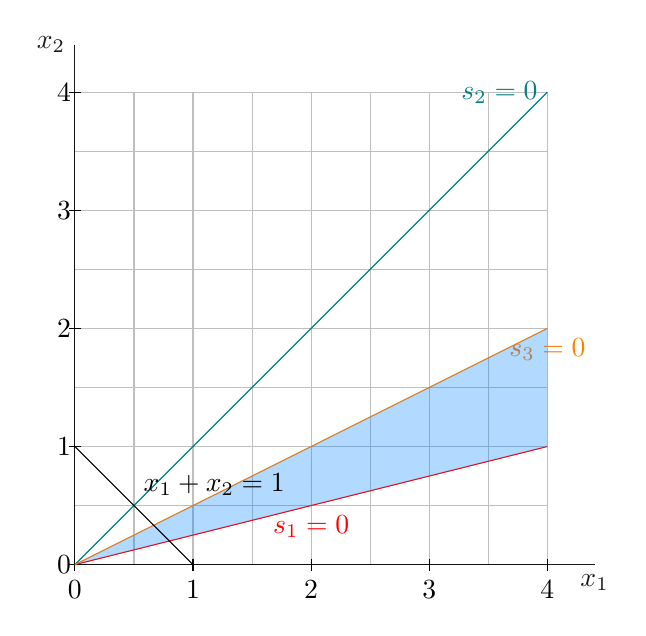
\begin{tikzpicture} [scale=1.5]
\draw[gray!50, thin, step=.5] (0,0) grid (4,4);
\draw[opacity=0.9] (0,0) -- (4.4,0) node[below] {$x_1$};
\draw[opacity=0.9] (0,0) -- (0,4.4) node[left] {$x_2$}; % option \draw[very thick,->]

\foreach \x in {0,...,4} \draw (\x,0.05) -- (\x,-0.05) node[below] {\x};
\foreach \y in {0,...,4} \draw (-0.05,\y) -- (0.05,\y) node[left] {\y};

\draw [red](0, 0) -- node[below] {$s_1=0$} (4, 1);
\draw [teal] (0,0)  -- (4,4) node[left, sloped] {$s_2=0$};
\draw [orange](0,0) -- (4,2) node[below, sloped] {$s_3=0$};
\fill[blue!50!cyan,opacity=0.3] (0,0) -- (4,2) -- (4,1) --  cycle;

\draw [black] (0,1)  -- node[above right] {$x_1+x_2 = 1$} (1,0);
\end{tikzpicture} \end{center}

\medskip Magnifying for clarity, and removing the $s_2=0$ (teal) line, as it is redundant, and marking the extreme points of the new feasible region, (4/5, 1/5) and (2/3, 1/3), with red boxes, we have:

\begin{center}  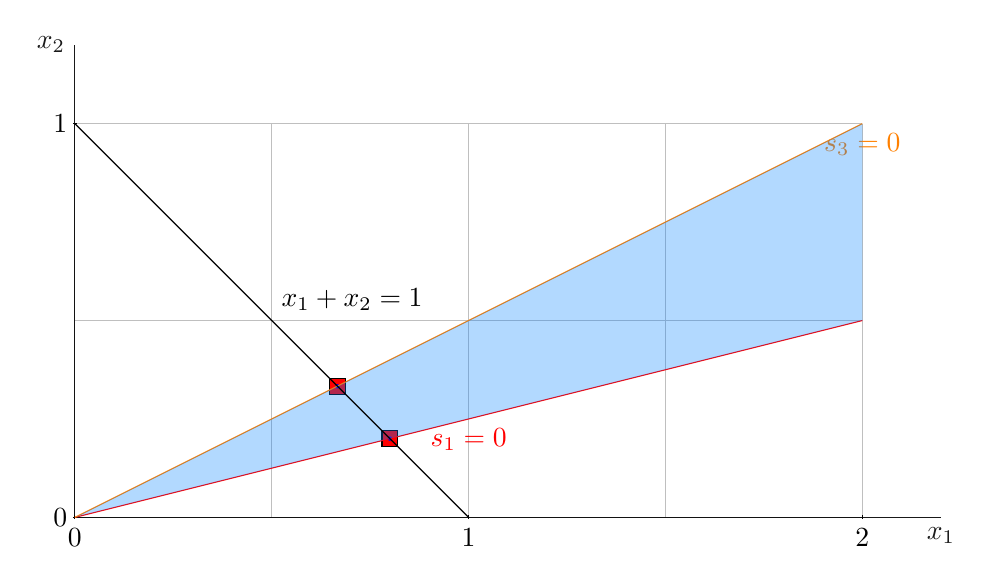
\begin{tikzpicture}[x=50mm, y=50mm]
\draw[gray!50, thin, step=.5] (0,0) grid (2,1);
\draw[opacity=0.9] (0,0) -- (2.2,0) node[below] {$x_1$};
\draw[opacity=0.9] (0,0) -- (0,1.2) node[left] {$x_2$}; % option \draw[very thick,->]

\foreach \x in {0,...,2} \draw (\x,0.005) -- (\x,-0.005) node[below] {\x};
\foreach \y in {0,...,1} \draw (-0.005,\y) -- (0.005,\y) node[left] {\y};

\filldraw[fill=red] (0.8-0.02,0.2-0.02) rectangle (0.8+0.02,0.2+0.02);
\filldraw[fill=red] (0.667-0.02,0.333-0.02) rectangle (0.667+0.02,0.333+0.02);
\node[fill=blue,circle,inner sep=0.02cm] at (0.8,0.2) {};
\node[fill=blue,circle,inner sep=0.02cm] at (0.667,0.333) {};

\draw [red](0, 0) -- node[below] {$s_1=0$} (2, .5);
\draw [orange](0,0) -- (2,1) node[below, sloped] {$s_3=0$};
\fill[blue!50!cyan,opacity=0.3] (0,0) -- (2,.5) -- (2,1) --  cycle;
\draw [black] (0,1)  -- node[above right] {$x_1+x_2 = 1$} (1,0);
\end{tikzpicture} \end{center}

The extreme directions are thus (4/5, 1/5) and (2/3, 1/3). \\


